\documentclass[10pt]{article}

\usepackage[T1]{fontenc}
\usepackage[utf8]{inputenc}
\usepackage[brazilian]{babel}
\usepackage{lipsum}
\usepackage{booktabs}
\usepackage{subcaption}
\usepackage{tabularx}
\usepackage{amsmath, amssymb}
\usepackage{import}
\usepackage{bm}
\usepackage[acronym, section=section]{glossaries}
\usepackage{listings}
\usepackage{indentfirst}
\usepackage{geometry}
\usepackage{graphicx}
\DeclareUnicodeCharacter{0301}{*************************************}
\DeclareUnicodeCharacter{0303}{*************************************}
\geometry{
	a4paper,
	total={170mm,257mm},
	left=20mm,
	top=20mm,
}

%%%Author definitions
\newcommand{\executeiffilenewer}[3]{%
	\ifnum\pdfstrcmp%
		{\pdffilemoddate{#1}}%
		{\pdffilemoddate{#2}}%
		>0%
			{\immediate\write18{#3}}%
	\fi%
}

\newcommand{\includesvg}[2][]{%
	\executeiffilenewer{#1#2.svg}{#1#2.pdf}%
	{inkscape -z -D --file=#1#2.svg --export-pdf=#1#2.pdf --export-latex}%
	\subimport{#1}{#2.pdf_tex}% s
}
\newcommand{\test}[2][]{
	% \immediate\write\{inkscpe}
}

\title{\textbf{Proposta de Trabalho Final\\ Método de Diferenças Finitas no Domínio do Tempo}}
\author{Tiago Vilela Lima Amorim}
\date{26 de Janeiro, 2021}
% \newacronym{FDTD}{FDTD}{Finite Difference Time Domain}
\newacronym{PDE}{PDE}{Partial Diferential Equation}

% \makeglossaries

\begin{document}
\maketitle
\section{Proposta}%
Dada a similaridade entre a equação de Shrödinger e a equação da onda, é possível controlar ondas eletromagnéticas dentro de estruturas periódicas de forma análoga ao controle de elétrons em semicondutores. Para tanto, existem técnicas para análise de \textit{band gaps} em cristais fotônicos utilizando tanto métodos baseados em Diferenças Finitas no Domínio do Tempo (FDTD, Finite-Difference Time-Domain) \cite{Lumerical_FDTD,shaobin_fdtd_2006} quanto Diferenças Finitas no Domínio da Frequëncia (FDFD, Finite-Difference Frequency-Domain) \cite{guo_photonic_2004,hanif_fdfd_2011}.
Propõe-se, portanto, o desenvolvimento de um programa baseado em diferenças finitas para análise de \textit{band gaps} em cristais fotônicos.


\section{Motivação}%
Tese de doutorado focada na aplicação de técnicas numéricas na análise de cristais fotônicos e metamateriais. Possibilidade de utilizar os resultados obtidos neste trabalho em estudo comparativo com técnicas sem malha e de elementos finitos.
\section{Desafios}%
\begin{itemize}
	\setlength\itemsep{0em}
	\item Formulação no domínio da frequência;
	\item Condições de contorno periódas;
	\item Complexidade teórica.
\end{itemize}
\section{Resultados Esperados}%
Espera-se, ao final do trabalho, o desenvolvimento de um programa baseado no método de diferenças finitas que permita a análise de \textit{band gaps} em cristais fotônicos.
\begin{figure}[ht]
	\begin{subfigure}{.5\textwidth}
		\centering
		% include first image
		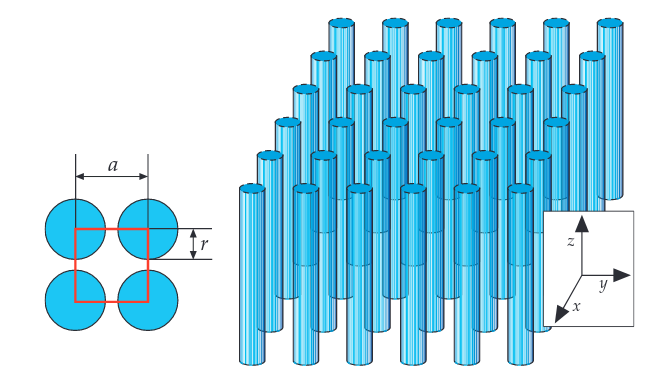
\includegraphics[width=.83\linewidth]{images/structure.png}
		\caption{Exemplo de cristal fotônico a ser estudado.}
	\end{subfigure}
	\begin{subfigure}{.5\textwidth}
		\centering
		% include second image
		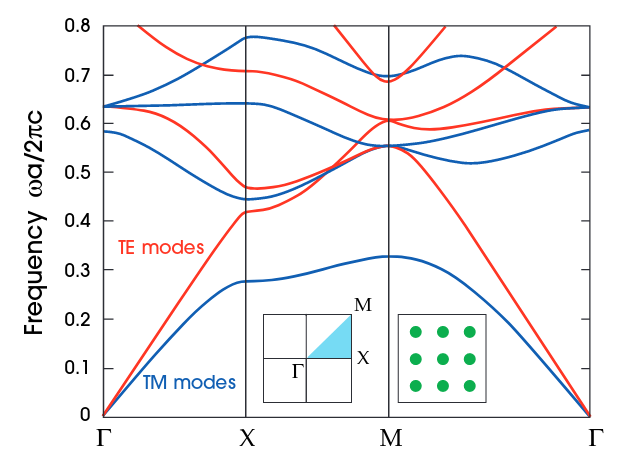
\includegraphics[width=.65\linewidth]{images/result.png}
		\caption{Resultado a ser obtido.}
	\end{subfigure}
	\caption{Imagem ilustrativa dos resultados a serem obtidos. (Figura emprestada de \cite{joannopoulos_photonic_2008}.)}

	\label{fig:fig}
\end{figure}

% \begin{figure}[h]
% 	\centering
% 	\def\svgwidth{0.8\columnwidth}
% 	\includesvg[figures/]{fig_ex1a}
% 	\caption{Circuito simulado: \textit{stripline}.}
% 	\label{fig:fig_ex1_stripline}
% \end{figure}
\bibliography{proposal}
\bibliographystyle{ieeetr}

\end{document}

